% !TEX root = ../main.tex


%%%%%%%%%%%%%%%%%%%%%%%%%%%%%%%%%%%%%%%%%%%%%%%%%%%%%%%%%%%%%%%%%


 \section{Evaluation of different methods}
 In this section we compare and evaluate different methods discussed in previous section and explain the consequences regarding each method to the users and developers of Dapps.
 \subsection{Criteria}
 There are some characteristics that can help the designer to decide which method should be used on the system and add upgradeability to the Dapp. In this part we pencil out these criteria and evaluate different methods based on these criteria. In this part we describe and specify what it means that each row of our table receives a full dot (\full), partial dot (\prt), or nothing. 
 
\subsubsection{Can replace entire logic}
An upgradeability method in which the admin is able to replace the entire logic of the system earns a full dot (\full) otherwise it receives nothing.

\subsubsection{No need to migrate state from old contract}
In some patterns, there is no need to collect data from the old version and push it to the new contract which receive a full dot (\full). On the other hand, patterns which required to migrate data from old version receive nothing.

\subsubsection{User endpoint address not changed}
In some upgradeability methods, after the upgrade process, users must call a new contract address to use the Dapp. It is equivalent to having 2 different Dapps at the end of the upgrade. Alice uses Dapp X which uses one of the upgradeability patterns at address A before the upgrade. After upgrade, she may be unaware that upgrade happened and use the previous address (receive full mark (\full)) or she may need to use address B instead which receive nothing.

\subsubsection{No need to instrument source}
Upgradeability patterns in which the developers do not need to change any part of the original code to add the upgrade method receives nothing. The methods in which the developers do not need to change the whole code but should add a proxy contract or change just one component of the system receive half dot (\prt) and patterns in which the developers should change the whole code to add upgradeability receive full mark (\full).


\subsubsection{No need to deploy a new contract}
In some upgradeability patterns, the admin needs to deploy a new smart contract in the process of upgrade which receives nothing. Upgradeability methods which do not need to deploy a new contract for the process of upgrade receive a full dot (\full).

\subsubsection{No indirection}  
Indirection happens if the first external message need be forwarded from a contract to another using one of the \texttt{CALL}, \texttt{STATICCALL}, or \texttt{DELEGATECALL} opcodes. Upgradeability methods that do not need any indirections receive a full dot (\full). An upgradeability pattern that contains indirections which adds an extra gas because of adding one or more layers of indirection awarded nothing. An upgradeability method in which not all but just a portion of the incoming transactions need indirection receive half dot (\prt). 


\subsubsection{No downtime to upgrade}
Patterns which have a downtime of the Dapp in the upgrade event receive full dot (\full) otherwise it receives nothing. 

\paragraph{Function Selector Clashes Risk}
Upgradeability methods in which the developer should take care of function selector risks due to the using of \texttt{DELEGATECALL} opcode receive full dot (\full), otherwise receive nothing. 

\paragraph{Storage Clashes Risk}
Upgradeability methods in which the developer should take care of storage clashes risks in two contracts due to the using of \texttt{DELEGATECALL} opcode receive full dot (\full). 



%%%%%%%%%%%%%%%%%%%%%%%%%%%%%%%%%%%%%%%%%%%%%%%%%%%%%%%%%%%%%%%%%%%%%%%%%%%%%%%%%%%%%%%%%%%%%%%%%%%
%%%%%%%%%%%%%%%%%%%%%%%%%%%%%%%%%%%%%%%%%%%%%%%%%%%%%%%%%%%%%%%%%%%%%%%%%%%%%%%%%%%%%%%%%%%%%%%%%%%
\subsection{Consequences}
In this section we discuss about the consequence of each upgrade methods regarding the criteria we mentioned in the previous part in users and developers that want to use the upgradeability pattern or uses a Dapp that uses one of the mentioned patterns.

\subsection{Speed of an Upgrade}
Upgrade events of a Dapp consists of two different processes. First a way to come to an agreement to a change, and then a way to implement and execute the change. The First part depends on the reason behind the upgrade. If the upgrade is to patch a bug, then the process to come into agreement is very fast but if the goal behind upgrade is to add new functionality or change a logic, it usually starts with a proposal and after the discussion if the agent that responsible for the decision agree with the proposal, the execution part will be started. We won't discuss about the first process because it depends on the type of agent that is responsible for the upgrades. The types of agents will be discussed in details in further sections which are EOA, Multi-sig and Decentralized Governance Voting system. 

After coming into agreement about the change, the speed that the upgrader can implement and execute the upgrade depends on three main criteria discussed above; \textit{Need to migrate state from old contract} , \textit{No need to migrate state from old contract}, and \textit{having a downtime in the upgrade process}.
 
\textit{Parameter change} method is the fastest way to execute the upgrade because there is no need to deploy a new contract, and no need to migrate state and no downtime in the system.
\textit{Component change} method change is not as fast as Parameter change method but faster than other types because the upgrader needs to deploy a specific smart contract which is a small component of the system and also update an address variable inside the main contract that points to that specific component and change it to the address of the new version of that component. But there is no need to migrate data and there is no downtime needed for this upgrade method.

\textit{Migration} method has a slow upgrade process. The reason is that the upgrader needs to deploy a new contract and also the upgrader or users should transfer the data from old version to the newer version. In most Migration processes the developer team deploy a \textit{Migrator} contract and users should use this Migrator contract to withdraw their funds/data from the previous version and move it to the newer version. But, there is no downtime in the Dapp and no need to change a state variable.

\textit{Call-based} and \textit{DelegateCall-based} are very similar to each other in the speed of upgrade. These two are not as quick as \textit{Retail changes} because the developer needs to implement and deploy the \textit{whole logic} contract to the blockchain and then change the pointer addresses inside the storage/proxy contract to the newer version. \textit{Diamonds} is very similar to these two but because Diamonds is a modularized pattern, in the event of upgrade we need to just implement and deploy one module which is related to the functions we want to change. So, the speed in Diamonds is similar to Component change methods.
On the other hand these two approaches are faster than \textit{Migration} because as mentioned before, there is no need to migrate data. There is no downtime in these methods.

\textit{Metamorphic} method is the slowest way to upgrade a system which uses this method because similar to the Migration plan there is a need to deploy a contract and migrate the state to the newer version but there is a difference between these two. In Metamorphic method the upgrader first should \textit{Self-Destruct} the previous version in a single transaction and after that transaction send a contract creation transaction to deploy the newer version. Because self destruct happened at the end of the transaction, the process of upgrade happens on two different transactions which is a downtime to the system. This downtime could be a gap between order of the two transaction in a single block or could be gap between blocks that these two transactions included into blockchain. 



\subsection{Cost of Upgrade}

 One of the main differences between upgradeability approaches is how much does the upgrade process costs for the upgrader and users. The cost of upgrade mostly depends on three criteria explained above; need to deploy a new contract, need to migrate a the state to newer version, and need to change a state variable.

 \textit{Parameter change} method is the cheapest method in the upgrade event because there is no need to deploy a new contract or migrate data but just need to change a state variable.

 \textit{Component change} is in the middle because there is a need to deploy a new contract (however it is cheaper comparing to methods in which we should deploy the whole logic), and change an address pointer variable but there is no need for data migration.

 \textit{Migration} plan is very expensive in the upgrade event because we need to deploy a new contract and migrate the data from the old version which is very expensive. But no need to change any state variables.

 \textit{Call-based} and \textit{DelegateCall-based} are very similar to each other in the cost of upgrade which is more expensive than component change but cheaper than migration. In both the upgrader must deploy the a contract containing the whole logic and change an address pointer inside storage/proxy contract. But there is no need to migrate the whole data.
 
 \textit{Diamond}'s cost of upgrade depends on the upgraded needed for the system. It is very similar to Delegate-based pattern but if there is a need to change some functions that are not in one module (faucet) of the system then we need to deploy more than one smart contract in the event of upgrade and so it is more expensive than doing upgrade comparing to Delegatecall-based pattern (however we do not need to deploy the whole logic but deploying a contract to ethereum blockchain is the most expensive action we have in EVM).

 \textit{Metamorphic} method is the most expensive method we have because we need to deploy a new contract, migrate data to the newer version and also we need to self destruct the previous version before the upgrade event which adds cost to the upgrade process.

\subsection{Gas overhead for users}
Sometimes in upgradeability patterns, we have a tradeoff between adding a feature to the pattern to improve it and increasing the cost for users that want to interact with our Dapp.

In patterns that needs indirection, such as \textit{Call-based}, \textit{Delegatecall-based}, \textit{Diamonds} and \textit{Component change} pattern we are adding a cost to the users because for all or some of the transactions to the Dapp, our system needs to forward the calls to another contract using Call or Delegatecall opcode to the users. 
Also in \textit{Delegatecall-based} and \textit{Diamond} pattern to mitigate the function selector clashes or storage clashes we need to add some checks to our code which also increases the cost of interacting with the Dapp. \textcolor{red}{We can compare all patterns like UUPS or transparent proxies in term of gas overhead here}.

Also there are some other ideas that addresses some limitations of a upgradeability pattern but increases the cost for users. For instance in \textit{Call-based} approach one of the problems is that after upgrade users should use a new address for using the Dapp but adding a \emph{Registry} contract can help to mitigate this. Using Registry contract, all other contracts should ask the registry to find out the latest version of the contract and then calls to the newer version which adds a gas cost to the users. 
% TODO: nice article: https://forum.openzeppelin.com/t/a-more-gas-efficient-upgradeable-proxy-by-not-using-storage/4111

 
 \subsection{Useability}
 Upgradeability patterns differ in term of Useability and it depends on three criteria explained above; \textit{User endpoint address changed}, \textit{Need to migrate state from old contract} and \textit{Downtime in upgrade events}.

Patterns in which the endpoint address is changing after upgrade event, \textit{Migration} and \textit{Call-based} is not user friendly because each time that the upgrade happened, the user must use the newer address. So make awareness about theis change is a hard action and need to socially interact with the users and make them aware of the change. We have two main type of users in the Dapp ecosystem, normal user or another smart contract (Dapp) that uses our system. Regular users which uses the official interface (website) of the project may do not sense any changes but users that work with the smart contract directly or via their own interface or other Dapps that uses the smart contract must have a way to upgrade the address they uses to use the newer version and if they did not implement a way to upgrade this address then their Dapp will face problems. So these patterns are make problems for composablility of the ecosystem.

In \textit{Migration} plan, in most cases of upgrade events the users are responsible for the migration of data. For instance, the user must withdraw the fund and use a \textit{Migrator} contract to push the data into the newer version which add costs to the user and it is not user friendly. This is one reason that make the Migration plans very hard because some users are not doing the process of migration and stay on the previous version which is like having a fork for the Dapp in side of the Dapp team. We see this happened on Uniswap V2 and V3.

In \textit{Metamorphic} pattern as mentioned before there is a downtime during the upgrade. So users cannot work with the Dapp on that exact time which is not user friendly.

\subsection{Dealing with two different new versions}
In \textit{Migration} and \textit{Call-based} pattern we will come up with two different Dapps. So a decision must be made for the previous version. One possible choice could be shutting down the old version. It can be done by self-destructing the old version, or by pausing mechanism which will be explained in further sections. In migration plan it is not regular to stop the previous version because in most migration plans, users are responsible to move their funds and data from the previous version to the new one and we cannot force them to do that, so we cannot stop the smart contract. 

The other option could be having a mechanism that after the upgrade, all calls to the previous version just be forwarded to the newer version which add costs and have some limitations like we cannot call the new functions defined in the newer version using the old version. This option is doable in Call based patterns. The other problem of this option is that if we upgrade a system more than one time then the calls to the first version should be indirected through lots of contracts to reach to the newer version. Also it adds complexity because developers must maintain more than one contract~\cite{ToBantiPattern}.


 \subsection{System Complexity} \label{sysComplexity}

 Using upgradeability patterns will add to complexity of our system but the degree of complexity varies and depends on the pattern. 
\textit{Parameter Change} method does not change the system in general but just adding a mechanism to change pre-specified variables in the system. The most important issue about the Parameter change method is that the developer team must limit the boundary of these parameter for the security of the system. For instance in MakerDao platform, Stability fee is changeable but if this variable be changed to \%100 then the whole system will be halted.

\textit{Component Change} pattern is very similar to the Parameter change but here a whole component could be changed and finding the safe boundary of changes and limiting this boundary is a bit harder.

\textit{Migration} plans for upgradeability does not change any complexity to the system because we do not need to change any part of system to add this type of upgradeability to it. The only important issue regarding this pattern is that we must be sure that there is a way to collect data from the old version like having getter functions for reading data and also having a withdraw function for users to collect data and funds from previous version and push or deposit it to the newer version.

Using \textit{Call-based} patterns adds higher degree of complexity to the system compared to previous patterns. As discussed before in this pattern we must be sure that the storage and logic contract is divided and there is not any storage variable inside the logic contract. This is one of the main security issues that found in the Dapps using this pattern regarding Trail of Bits company reports~\cite{ToBantiPattern}. As mentioned before to add a way to storage contract to define new variables, developers uses the Eternal Storage pattern for their storage contract which is very hard to apply for complex data structures in Ethereum such as mappings or structures. This is another source of complexity using Call-based pattern.

\textit{Delegate-call} pattern adds complexity to the code because of using \textit{Delegate-call} opcode in its logic. As mentioned above because of using this opcode, the developer should take care of storage clashes and also function selector clashes. Other than these two there are some other limitations and risks of using this patterns. For instance, we cannot have a \textit{Constructor} function on the logic contract (implementation contract) because constructor functions is used to initialize specific variables at deployment time and if we have a constructor inside the logic, then storage of implementation contract will be changed and not storage of proxy contract. To mitigate this problem we can add a regular function named \textit{Initialize} function inside the implementation and make sure that this function can be called \emph{once} to act just like a constructor function. Using initialize function brings some security risks that we will explain in further sections.

\textit{Diamonds} pattern is very similar to the Delegate-call based patterns and have the same risks but this pattern is more complex because here we have different implementation contract for a single proxy and we should be sure that all of these implementation contracts share the same storage layout otherwise we will have a storage clash problem. 

\textit{Metamorphic} pattern is proposed recently and not well-tested yet. There are some risks to this pattern as well. We should be sure that we have a mechanism to self-destruct the contract. Otherwise if we cannot self-destruct the current contract we cannot redeploy a new version and so our contract won't be upgradeable. The other important issue related to Metamorphic pattern is that the developer must know that each time they want to upgrade the system the whole storage will be wiped out and need to re-initiate the whole state after re-deployment. 


 %%%%%%%%%%%%%%%%%%%%%%%%%%%%%%%%%%%%%%%%%%%%%%%%%%%%%%%%%%%%%%%%%%%%%%%%%%%%%%%%%%%%%%%%%%%%%%%%%%%%%%%%%%%%%%%%%%%%%%%%%%%%%%%%%%%%%%%%%%%%
 %%%%%%%%%%%%%%%%%%%%%%%%%%%%%%%%%%%%%%%%%%%%%%%%%%%%%%%%%%%%%%%%%%%%%%%%%%%%%%%%%%%%%%%%%%%%%%%%%%%%%%%%%%%%%%%%%%%%%%%%%%%%%%%%%%%%%%%%%%%%

\clearpage 

\section{Implementation detail of Finding The proxy contracts}

\subsubsection{Implementation}\label{findingProxies}
In this section we describe the processes of finding upgradeable proxy contracts explained in the previous section in detail of implementation and execution. 
Each block of Ethereum blockchain consists of transactions that processed in that exact block. To get all transaction details we need to replay the transaction and collect the data of execution of the transaction. Ethereum full archival node has a method, \textit{trace\_transaction}, that gives the \textit{Parity VM transaction traces} of the transactions executed on the specific block. This transaction traces are composed of \textit{actions}. Each action gives data about each specific part of the execution of the transaction and consists of the opcode instruction that is executed on that action and the input data relevant to the that instruction and also information about how it manipulates the state, memory or stack of the Ethereum Virtual Machine (EVM). 

Having the transaction traces for each block, we will search to find actions that consists of \textit{callType}. When an action has callType field it means that there is a call happened in that specific action, which means one of \textit{Call},\textit{Static Call} or \textit{Delegatecall} happened in that action. we picked actions that have \textit{callType} and this call type is \textit{delegate call}. Also each action has an \textit{input} element for messages that shows the call data (the data that is used for the calling the callee address). 
If the input element of the selected actions are equal to the input element of their previous action with the same transaction hash, it means the transaction passes a fallback function which delegate calls it to another contract. 
Because the input is not changed after the call it means that it passes a fallback function because the function selector (first four byes of the input) has not been changed which means the called function does not exists in the contract, so the fallback is called. Also the delegate call in the action shows that inside that fallback function there is a delegatecall that passes the whole message data to the target address contract. So, these contracts meet first condition described in the methodology part and these contracts are proxy contracts. We collect \textit{From address},\textit{To address} and the \textit{transaction hash} of these picked actions and pick the unique from addresses of this data. From address is the address of sender of transaction (proxy contract addresses), to address is the address which the proxy sends the transaction into (implementation contract addresses) and transaction hash is the transaction identifier that is used in Ethereum blockchain. 

As discussed before, these selected contracts are proxy contracts and not necessarily upgradeable proxy contracts. So, we need to filter the \textit{forwarders} from proxy contracts to find upgradeable proxy contracts. As mentioned in methodology section, the upgradeable proxy contracts must satisfy a condition; the admin of the contract should be able to change the target address. In other words, we should check if the target address inside the proxy contract is changeable or not.

There are five regular ways for the situation that the target address is fixed and not changeable on the contract:
\begin{enumerate}
  \item The target address is hardcoded in the contract without assignment to any variables
  \item The target address is saved in a constant variable type 
  \item The target address is saved in an immutable variable type and the deployer sets it via a constructor function
  \item The target address is defined in a storage variable, but there is no function or a way to change this address after contract deployment (neither in proxy contract nor in implementation contract)
  \item The proxy contract grabs the target address each time by calling another contract and there is no way on the callee contract to change this address
\end{enumerate} 

In the first three situations, the target address amount will be appeared on the runtime bytecode (the bytecode that is saved in the blockchain after deployment) of the smart contract. We can get the bytecode of each proxy contract that are collected from previous part using the \textit{eth\_getCode} method of a Ethereum archival node and check whether the target address is appeared on the bytecode or not. To have the target addresses we just need to collect The \textit{To addresses} that we collected on the previous part which are supposed to be the implementation addresses because the proxy contract delegate calls into these addresses. So we check if the target address is appeared on the bytecode of the proxy contract. If yes, these proxies are not upgradeable proxies and they are forwarder contracts because the address is hardcoded on the bytecode and cannot be changed after deployment. Finding the forwarders, we removed them from the list of the proxy contracts.

For the situation 4, we need other processes to check whether the implementation address is changeable or not. We need to design a filter to tell us if there is a way to change the target address after deployment or not. We will describe the filter in the later part of the paper, but for now let's assume that we have a module named \textit{Assignment Checker} that checks the code and tells us that whether there is a function inside the contract that the caller can change the \textit{target address} using the function. If yes we mark the contract as an upgradeable proxy contract because there is a way in the proxy contract to change the target address and point it to the new implementation contract and upgrade the system.

For the situation 5, we check the proxy contract to find whether each time before the delegate call, the target address inside the proxy contract is coming from an external call to another contract. If yes the we check the callee smart contract (a.k.a Beacon contract) that if the target address is changeable inside that contract or not. If it is changeable we mark the proxy as \textit{Beacon Proxy} otherwise it is a \textit{Forwarder}. 

But this is not the end of story. There is another proposed upgradeable proxy contract pattern, named Universal Upgradeable Proxy Standard (UUPS) also known as EIP-1822~\cite{uupsEIP} that described in the previous sessions. In this type of proxy contracts, the target address can be changed using the implementation contract and not the proxy itself. As mentioned before the code of the implementation contract is executed in the context of the proxy contract and so it will change the storage state of the proxy contract. If we have a function in the implementation contract that gives us the ability to change the storage slot of the target address, we can upgrade the system by calling that function of implementation contract through proxy itself. We couldn't catch this type of upgradeable contracts by the previous processes because we just checked if there is a function inside the proxy contract itself that can change the target address.

We can tackle this problem by first finding the storage slot of the target address inside proxy contract. Then by using the \textit{Assignment Module} to check if there is a function inside implementation contract which gives the admin right to change the target address. So first we should find the storage slot of the proxy contract in which the target address is saved. There are two EIPs out there that makes it easy to find these storage slots that suggested to be used to save target address for upgradeable proxies; EIP-1967 \footnote{0x360894a13ba1a3210667c828492db98dca3e2076cc3735a920a3ca505d382bbc} and EIP-1822 \footnote{0xc5f16f0fcc639fa48a6947836d9850f504798523bf8c9a3a87d5876cf622bcf7}, suggested randomly selected storage slots for target address to mitigate the overwriting on these slots. The UUPS contracts are usually using one of these two storage slots to save their target address.

The more general way to do this is not using these proposed slots from these EIPs for this process. The general way is to find the storage slot from the proxy contract and then check if admin can change this specific storage slot inside the implementation contract. But this way is not doable in large scale because in \textit{Assignment checker} module we need to decompile the bytecode which is time consuming for contracts that have a large bytecode. Implementation contracts are usually large pieces of codes. So, it is not possible to do this process in a large-scale for all proxy contracts that are found from the previous parts. This is the reason that we limit our filter to specific storage slots proposed in EIP 1967 and EIP 1822.

So for this part we use the remained proxy contract addresses from the previous part. First we select the contracts that their target address is saved on the mentioned storage slots and if the target address is saved on the slot, check the implementation contract to find variable regarding that storage slot defined in the implementation contract. Afterwards check if the variable is changeable in a function in implementation contract. If it is changeable, it means that the admin can upgrade the system using a function on the implementation contract, and so the proxy is an UUPS contract. 

The whole process is depicted on figure~\ref{fig:finderModule}.

\begin{figure}[t!]
  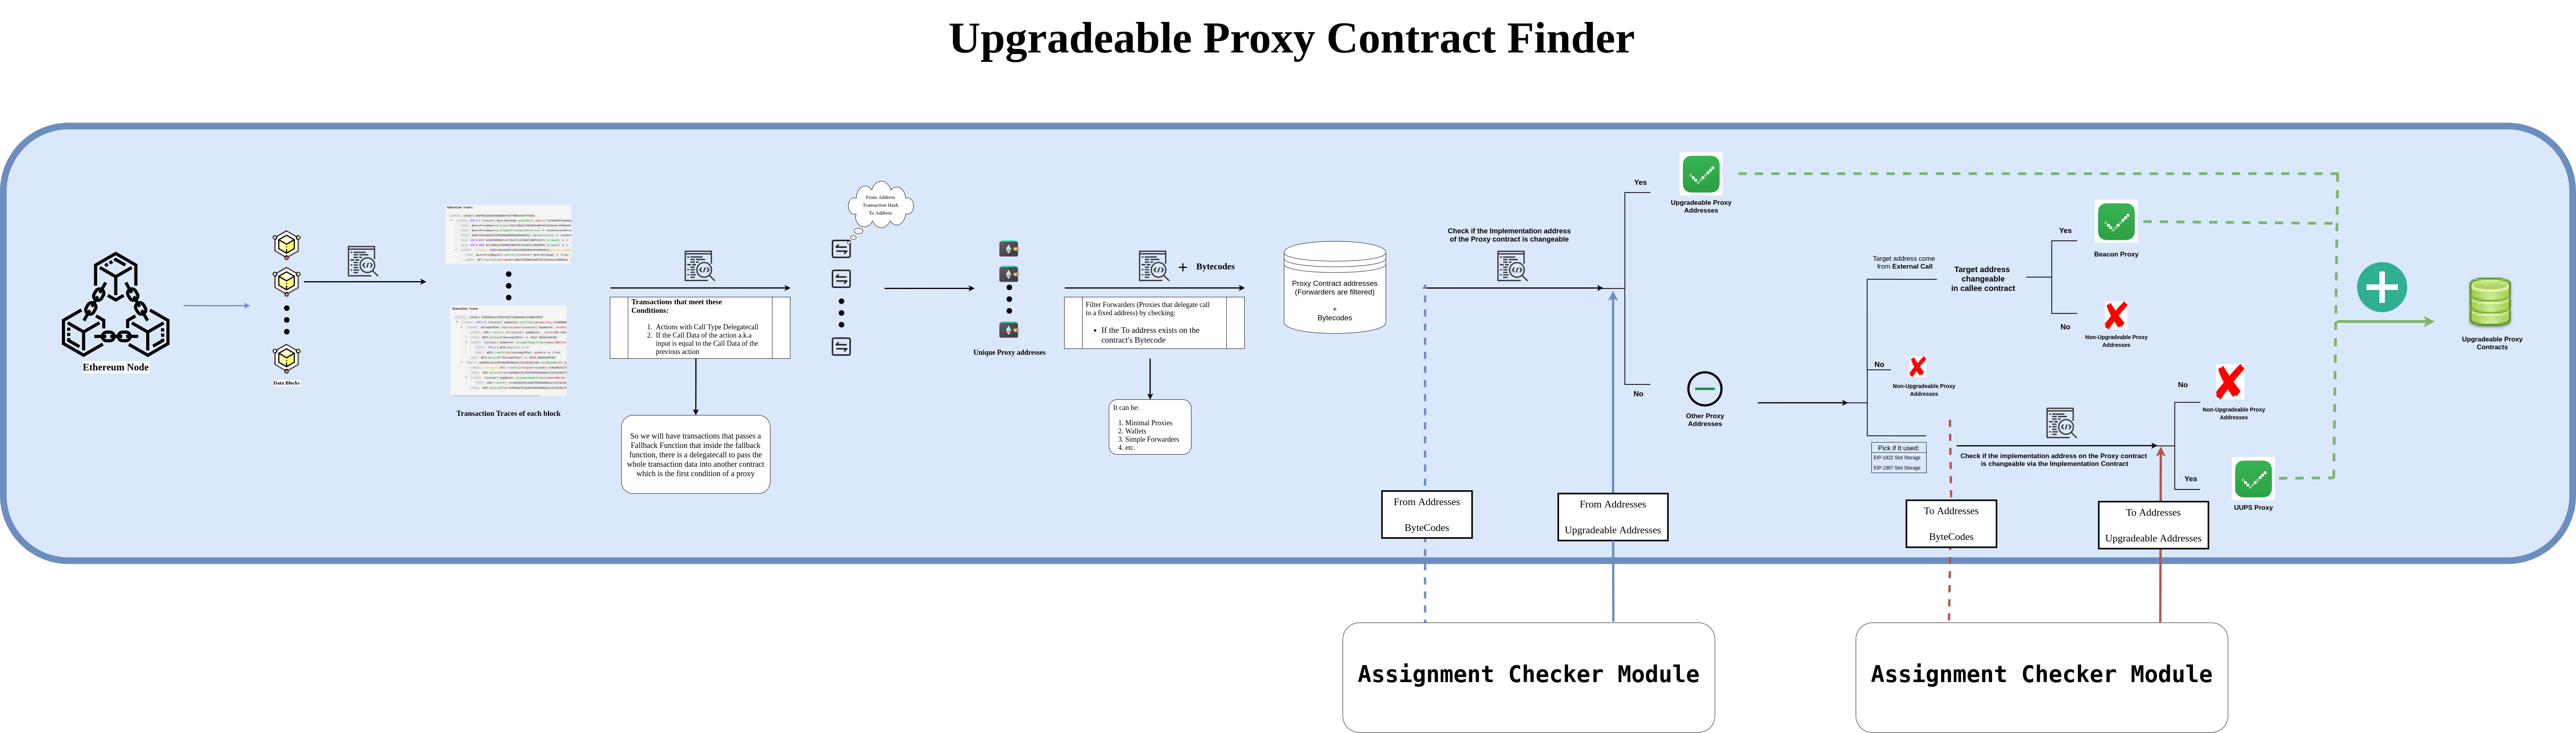
\includegraphics[width=0.8\textwidth]{figures/Upgradeability_finder1.png}\label{fig:finderModule}
  \caption{Upgradeability Proxy Contract Finder}
\end{figure}

\subsection{Assignment Checker Module}

As mentioned in the previous part, we need a module to check whether the admin can change target address on the proxy contract,using a function in the proxy contract, implementation contract or beacon contract. For this purpose the module must get the \textit{Bytecode} of the proxy,implementation or beacon address as input and find the variable name and also its storage slot of the target address. Then checks to find out is there any function inside the contract that gives the admin the ability to change the target address.

We use bytecode decompiler named \textit{Panoramix decompiler} \footnote{\url{https://github.com/palkeo/panoramix}} to decompile the bytecode into well-formatted python language codes. The decompiled code gives us all storage variables of the related contract and the storage slots of those variables in a function named \textbf{Storage}. On the other hand, the decompiled code will tell us if a function is \textit{Payable} or not. Among these Payable functions the one that does not have name or its name is fallback is the \textit{fallback} function of the contract. So we will try to find the line of code that \textit{Delegate Call} happened on it and collect these lines. Now that we have storage variable names and storage slots of these variables and also the line of code inside fallback that have the delegatecall, we will check to find the target address variables. We are doing that by checking if one of the storage variables inside Storage function is used in the line of code that contains delegate call. We will add them to an array of implementation addresses.
% or if there is a hash a text is inside the line of the code (if there is 'sha3' inside the line). 

There is two other steps here. First finding other variable names with the same storage slots as the implementation addresses we found from the first step by checking the Storage function and also finding another variables that being assigned to those implementation variables in some other part of the code. We will add these two type of variables to the implementation addresses as well.

Now that we have a list for implementation addresses, we will search through the code to find if any assignment happened to one of them. If yes we will pick the variables that is assigned to target variable and then check if this assignment happened in a specific function and to one of the inputs of that function. In this case this function will be the upgrade function because the caller of this function can upgrade the target address by calling this function with desired input. 

To summarize what we did, we find all possible variables in the code that can change the target address inside the contract and check if there is any function inside them that can assign new address to the target address variable.

The whole process is depicted on figure~\ref{assignmentFinder}.

\begin{figure}[t]
  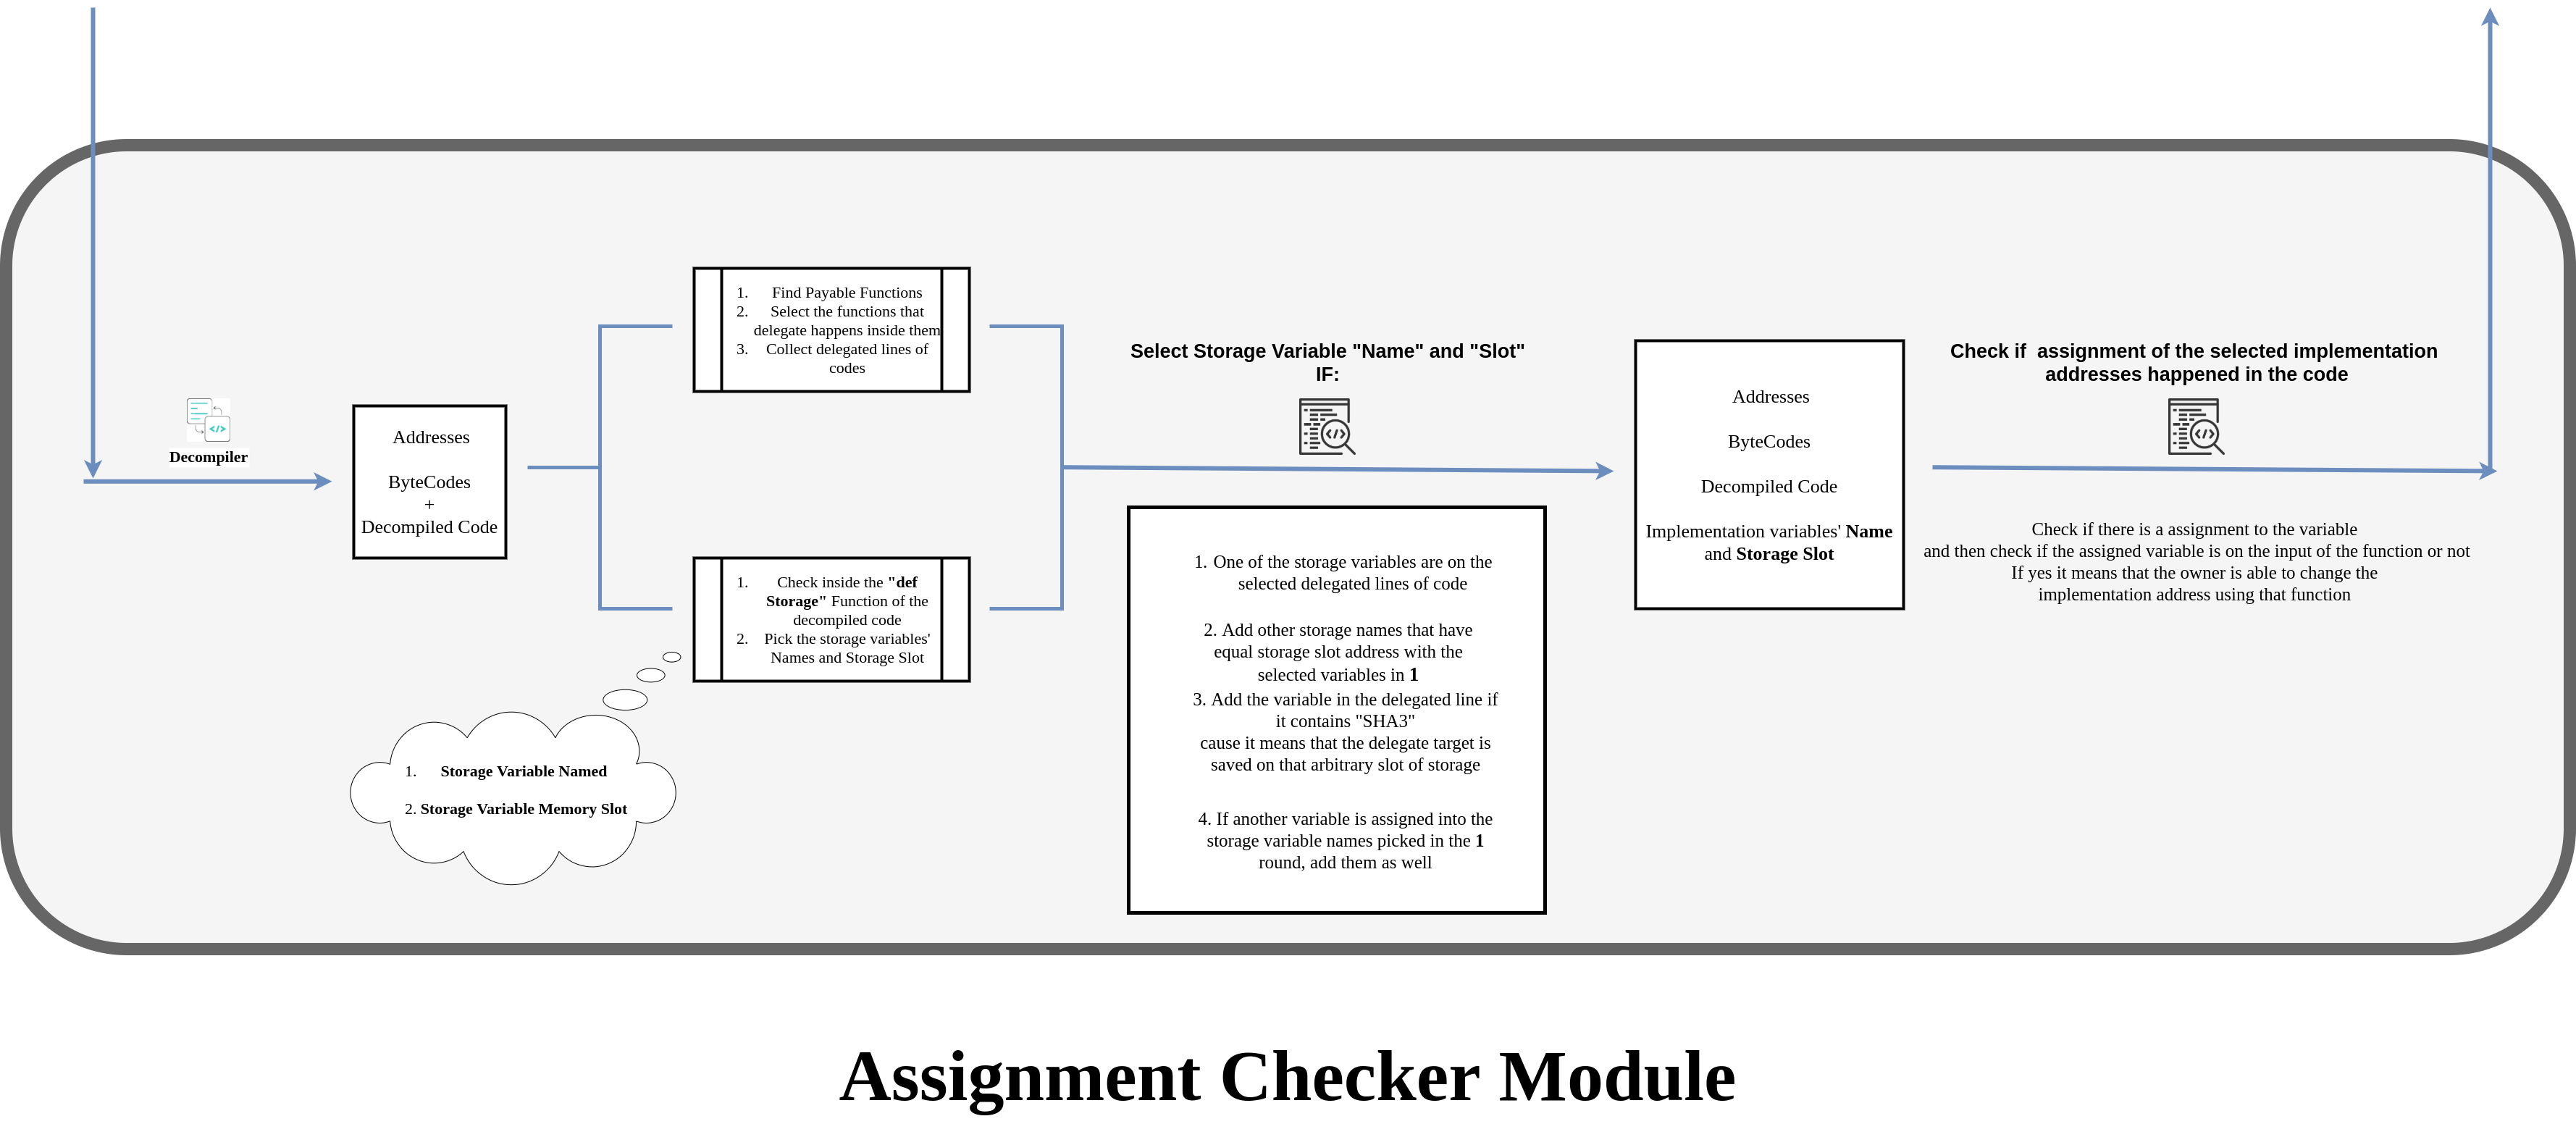
\includegraphics[width=0.8\textwidth]{figures/Assignment_finder.png}\label{assignmentFinder}
  \caption{Assignment CheckerModule}
\end{figure}

% = = = = = = = = = = = = = = = = = = = = = = = = = = = = = = = = = = = = = = = 

\clearpage
\section{Detailed Explanation of finding Admin types}
The whole process is depicted in the figure\ref{Admins}.

\begin{figure}
  \centering
  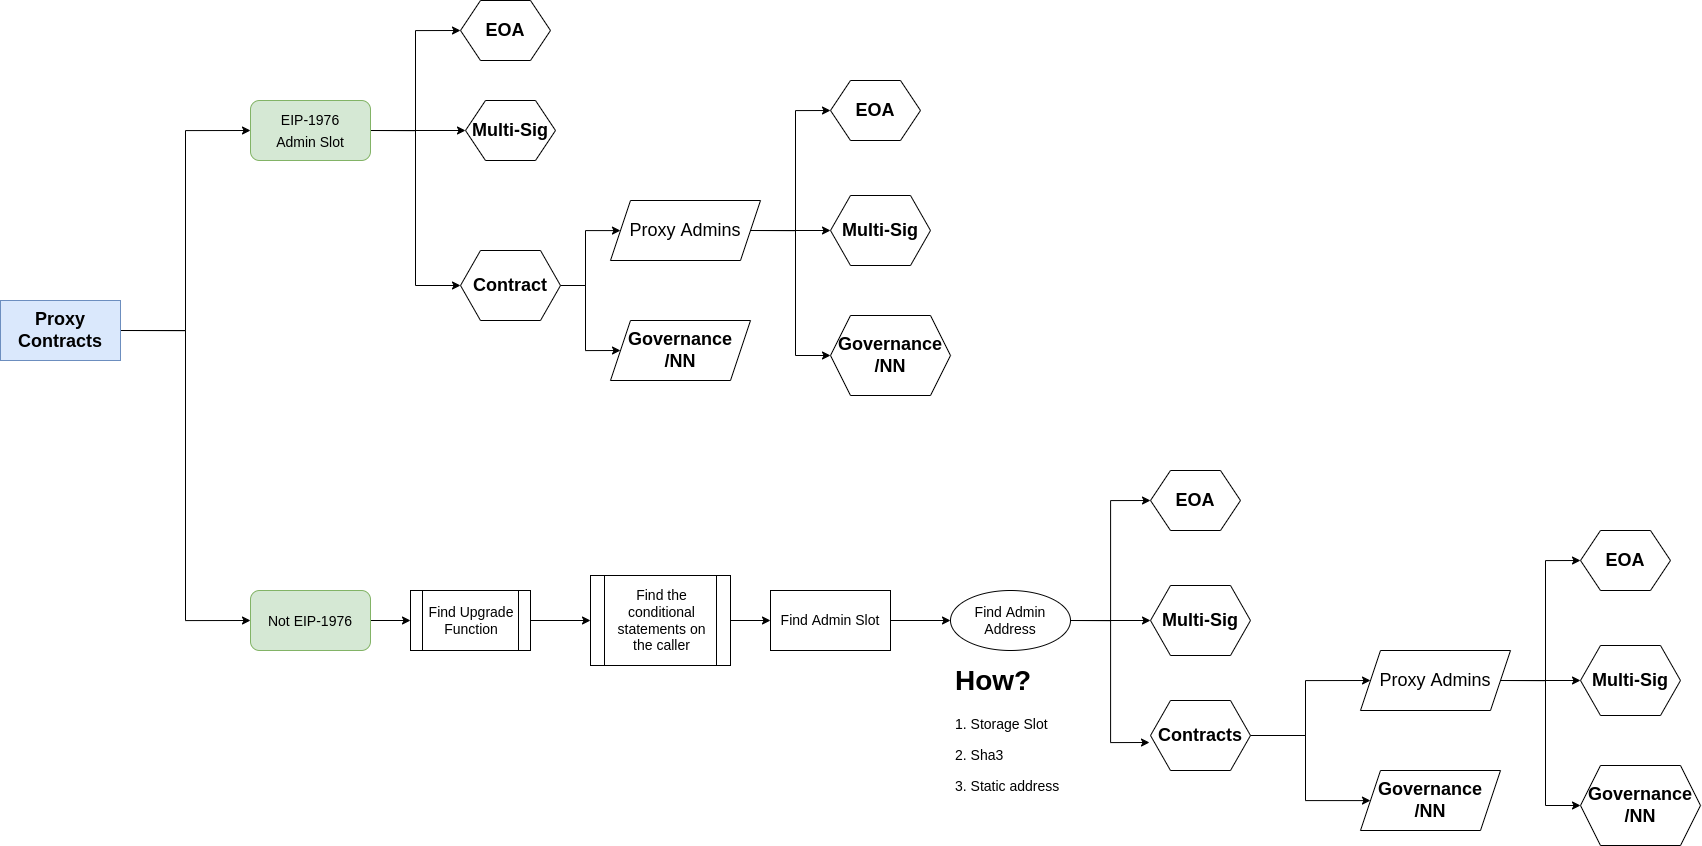
\includegraphics[width=1.0\textwidth]{figures/Admins.png}\label{Admins}
  \caption{Admin Types}
\end{figure}

\paragraph{EIP-1967.}As mentioned above EIP-1967~\cite{eip1967} suggested specific arbitrary slots for upgradeable proxy contracts to store implementation contract's address and \textit{Admin address}\footnote{Storage slot 0xb53127684a568b3173ae13b9f8a6016e243e63b6e8ee1178d6a717850b5d6103 for admin}.

In first step we use \textit{eth\_getStorageAt} method of an Ethereum full archival node to search the EIP-1967 specified storage slot for admins on our 7.3k proxy contracts. If the result of this method is non-zero it means that the proxy uses EIP-1967 standard because the specified storage slot is an arbitrary slot and one can store variable in this slot just by defining this slot which means that they used EIP-1967.

So, for non zero results, we capture the address which is the address of admin of the proxy. Now we try to find the type of these admin addresses. Having the address of the admin we use \textit{eth\_getCode} method to check the code of the admin account. If the code is empty, it means that this account is not a smart contract so it is an EOA. we find \textit{900} EOA admins that their proxy uses EIP-1967 standard.

The remained admin addresses are contract because their account keeps code. This contract can be multi signature smart contract wallets. The most widely used multi signature wallet is Gnosis Safe\footnote{\url{https://gnosis-safe.io/}} wallets. We automatically checked if the code of the admin address is the Gnosis wallet multi signature patterns. After picking Gnosis safe wallets we manually checked \%10 of the remained addresses to find if they used other patterns for their multi signature wallet and we found some other patterns (e.g. MultiSignatureWalletWithDailyLimit, etc.). After Finding all these types we checked the admin codes to see whether they are multi signature wallets. We find \textit{255} admin accounts that uses multi signature wallets as their admin.

There is another class of admin contracts named \textit{Admin Proxy} contracts. These admin proxy contracts are another layer of re-direction between the real admin and the Dapp's proxy contract. The admin proxy contracts are proxy contracts that redirect the messages from the real admin into the Dapp's proxy. The only person who can use admin proxy is the admin (a.k.a owner) of the admin proxy. So we first filter the admin proxy contracts using the codes we get from the previous part and then try to find the owner of the admin proxy contracts. The owner of admin proxy contract (the real admin) also can be EOA, Multi-sig or governance contract. Finding the owner of the admin proxy contract, we used \textit{eth\_getCode} method to check the code of these account and find out if they are EOAs or Multi-signatures or governance schemes. Doing this we find \textit{1202} EOA admin accounts and \textit{567} multi signature admins. We marked the remained proxy admin addresses as Governance/Not Known admin types and we have \textit{462} of them. There were also non admin proxy contracts which use EIP-1967 but they were not EOA or Multi signatures. We marked them as Governance/Not Known admin types and we have \textit{53} of them.


\paragraph{Non EIP-1967.}

For proxy contracts which not use EIP-1967, the problem is we don't know where the admin address is saved in the proxy contract's storage (what is the storage slot of the admin address). It can be saved in a storage slot of the contract or be hardcoded in the smart contract\footnote{There are some other possible ways to store the admin address for instance saving it in another contract and each time make an external call to get the address but to our knowledge this pattern is not widely used as a standard}. 

So there are two ways that the admin address is saved in the proxy contract. It can be saved as a storage variables or it can be hardcoded as a fixed address.

In storage variable case, the first question is in which storage slot the admin address is stored. So, the first step is to find the storage slot of the admin address variable. Also for the fixed address we should find the fixed address of the admin directly.

To find the slot of the storage variable in which admin address is saved, we first find the function in which the proxy can be upgraded. For finding the upgrade function we exactly do what we did in \ref{findingProxies} part. We first find the storage variable in which we saved the implementation address and then we find a function in which the implementation address can be changed using the inputs of that specific function. 

The upgrade function of a proxy contract is a critical function and the only account that can call this function should be the admin of the proxy contract. So, there should be an access control check inside the upgrade function to check whether transaction sender is equal to the admin address or not.
So, after finding the upgrade function we search for conditionals that checks the caller of the transaction and by doing that we can find the admin address or the storage variable in which the admin address is stored.


If the admin address is stored in a storage variable, then we should find the storage slot of that specific storage variable. For finding the storage slot we do what we did in \ref{findingProxies} part by using \textit{def storage} function of the decompiler and check the storage slot of the storage variable we found, and the admin address is saved on it. 
Now we have the storage slot of the admin address and we should start doing all the things we did for EIP-1967 in the previous part. 
In the EIP-1967 the storage slot for admin address was pre-specified and we do not need to find the slot but in this case we use the above methodology to find the slot but the further steps are the same as EIP-1967.
So, by using the \textit{eth\_getCode} method for admin address inside the storage slot we find above, we can check wether the admin is EOA, Multi-sig, Governance, Proxy admin or not known.
In this part we find \textit{1313} EOA addresses and \textit{104} multi-sig admins. Also by checking proxy admins we find \textit{92} EOA addresses and \textit{16} Multi signatures that uses proxy admin as a level of indirection. 

In another case the admin address may be stored directly in a specific arbitrary storage slots. In this type the compiler will specify the address using the \textit{sha3} hash notation. In this case same as above we find the conditional check on the transaction sender and then find the storage slot in that line and hash of that pre-specified string. 
By finding this arbitrary storage slot and doing the same processes we did in the previous part we find \textit{2} EOA addresses and \textit{10} Multi-sig addresses.

The only case that is left is proxy contracts, in which the address of the admin is hardcoded inside them. It very straight forward. We find the upgrade function and the access control check on the caller of the transaction and then pick the fixed admin address and do the same processes mentioned above to find the admin types. There are \textit{49} EOAs, \textit{36} multi-signature admins and \textit{160} governance and not known admin addresses. 

So, totally out of 7.3k proxy contract, \textbf{3558} are controlled by an EOA address, \textbf{988} are controlled by a multi signature wallet and \textbf{2924} addresses are governance controlled or our methodology could not find their type.



% = = = = = = = = = = = = = = = = = = = =
% = = = = = = = = = = = = = = = = = = = =
% = = = = = = = = = = = = = = = = = = = =


\begin{comment}
\subsection{Verified Smart Contract Based Analysis}
In this section we aim to shed light on these vital unanswered questions: 
 \begin{enumerate}
  \item How many of the existing Dapps on the Ethereum blockchain are upgradeable?
  \item Who can control these upgradeable Dapps (i.e who is the admin)? 
  \item In what extent the Dapp can be changed?
  \item What is the average frequency of updates on the Ethereum Dapps?
  \item How many times the admin of upgradeable contracts changes on average?
\end{enumerate}
To have analysis on Ethereum blockchain some widely used methodologies are Transaction-based analysis, Bytecode based analysis, Etherscan Verified Smart Contracts based analysis or combination of these methods. The first and second methodologies need to access to an Ethereum full archival node. But the last approach need to collect smart contracts from a third party service named Etherscan.io in which the Dapp developers are able to put their high-level language smart contracts which will be checked and verified from the bytecode of the Dapp on the Ethereum blockchain.

In the first attempt we conducted a measurement study based on verified smart contracts on Etherscan to find instances of OpenZeppelin upgradeable proxy contracts. OpenZeppelin is a team that built well-known libraries for ethereum developers. One of their is upgradeability plugins. There two different versions of the OpenZeppelin upgrade libraries: version 2.6 and version 3+. 
We used smart-contract-sanctuary~\cite{smart_contract_sanctuary} which is a data set of all ethereum smart contracts verified on Etherscan. For this analysis we analyzed 93,000 smart contracts that are deployed on the main Ethereum blockchain and verified their contracts on Etherscan. 

To find the smart contracts which used different versions of the OpenZeppelin upgradeability library, two different approaches are used. First, we used an Abstract Syntax Tree (AST) based similarity detector: Solidity Doppelgaenger~\cite{solidity-doppelganger}. We found 143 smart contracts that used version 2.6 and 125 version 3+ OpenZeppelin upgrade libraries. 

In another attempt, we used Regular Expression (regex) to find if the smart contracts on our data set used the interface (function and variable used on the code) of the each version of the OpenZeppelin libraries. The unique interface that used in each version of the OpenZeppelin libraries helps us to find them just by checking the interface. We found 922 contracts using V2.6 and 309 contracts using V3+. All results from AST-based detection was found on the interface detection results. So we used the results from interface detection for the rest of this part.

Now that we have the address of upgradeable smart contracts we can check how many times the upgrade happened for each and how many times the admin of the upgradeable contract is changed. For this purpose, OpenZeppelin libraries have used Ethereum Events on the functions in which the upgrade happens (Event "Upgraded") and the admin changes (Event "AdminChanged") and fired these events when the upgrade happened or the admin changed. We capture these events for each contract address using Etherscan Ethereum Log API service.

\begin{figure}[t]
  \centering
      \subfloat[OpenZeppelin V2.6]{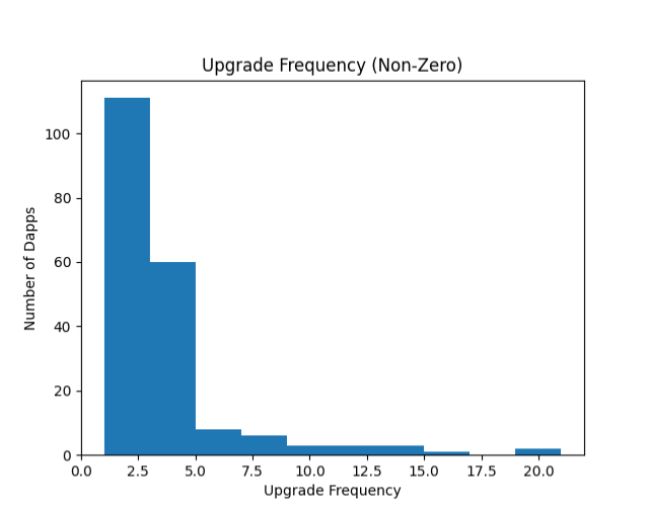
\includegraphics[width=0.45\columnwidth]{figures/UpgradeV26.png}\label{fig:upgradev26}}
      \qquad
      \subfloat[OpenZeppelin V3+]{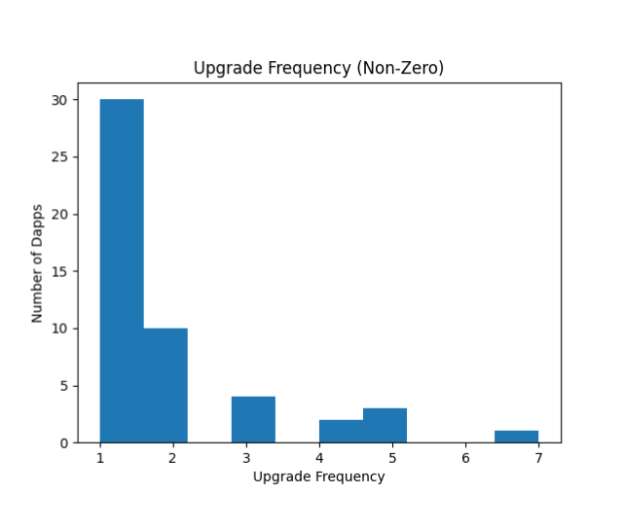
\includegraphics[width=0.45\columnwidth]{figures/upgradev3.png}\label{fig:upgradev3}}
  \caption{Number of Dapps (y-axis) over number of upgrades (x-axis) \label{fig:upgrade}}
\end{figure}
\begin{figure}[t]
  \centering
      \subfloat[OpenZeppelin V2.6]{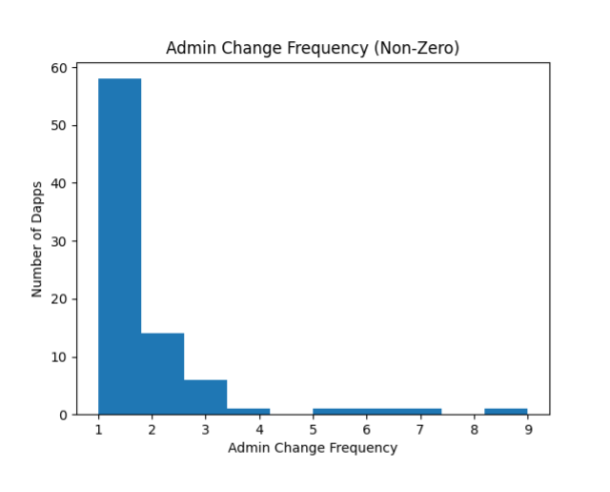
\includegraphics[width=0.45\columnwidth]{figures/Adminv26.png}\label{fig:adminv26}}
      \qquad
      \subfloat[OpenZeppelin V3+]{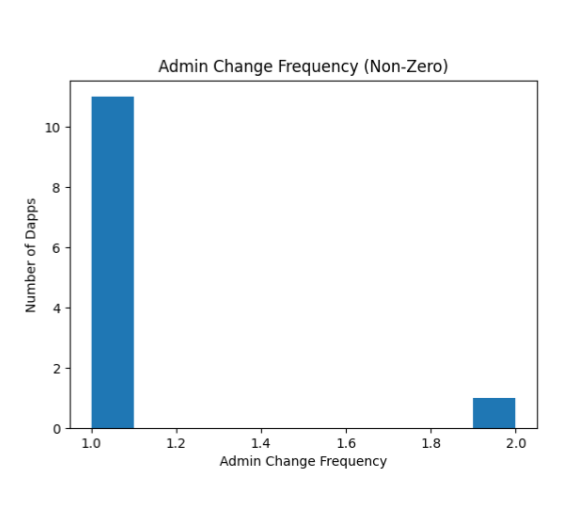
\includegraphics[width=0.45\columnwidth]{figures/Adminv3.png}\label{fig:adminv3}}
  \caption{Number of Dapps (y-axis) over number of Admin Changes (x-axis) \label{fig:admin}}
\end{figure}
The results for each version is:
\begin{itemize}
  \item For V2.6 (922 contracts):
  \begin{itemize}
    \item Upgrade Happens (see figure~\ref{fig:upgradev26}):
    \begin{itemize}
      \item 110 with One Upgrade, 60 with Two Upgrade, 2 with 20 upgrades, 5 with Five upgrade, 4 with 7 Upgrades, 3 with 10,12,15,16 Upgrades, 1 with 16 upgrades
    \end{itemize}
    \item Admin Change Happens (see figure~\ref{fig:upgradev3}):
    \begin{itemize}
      \item 57 with One Change, 14 with Two change, 4 with Three change, 1 with 4 changes, 1 Dapp with 5, 6,7,9 Changes
    \end{itemize}
  \end{itemize}
  \item For V3+ (309 contracts):
  \begin{itemize}
    \item Upgrade Happens (see figure~\ref{fig:adminv26}):
    \begin{itemize}
      \item 30 with One Upgrade, 10 with Two Upgrade, 4 with Three upgrade, 2 with 4 Upgrades, 3 with 5 Upgrades, 2 with 7 Upgrades
    \end{itemize}
    \item Admin Change Happens (see figure~\ref{fig:adminv3}):
    \begin{itemize}
      \item 11 with One Change, 1 with Two change
    \end{itemize}
  \end{itemize}
\end{itemize}

\end{comment}

% = = = = = = = = = = = = = = = = = = = =
% = = = = = = = = = = = = = = = = = = = =
% = = = = = = = = = = = = = = = = = = = =

\section{Attacking Universal Upgradeable Proxy Standard (UUPS) contracts} \label{sec:attackUUPS}
In the previous sections \ref{sysComplexity} (in Delegate-call section) we discussed that the implementation function should not contain \textit{constructor} function and instead of that there should be regular function namely \textit{Initialize} function that can be called just once and has the same functionality as constructor function. So the contract creator must call initialize function through proxy contract quickly after deploying the proxy contract. The Initialize function does not have any access control because it is considered to be called once and this function is responsible to define the owner so before calling this function we don't have the owner's address to check it for access control of the function. This is the main reason that there should be a check to be sure that this function can just be called once and not more. Regularly, the deployer (the dev team) will define and initialize the owner of the contract (address which have the control of upgrading the system) via initialize function. So if the initialize function can be called more than once, or the deployer do not initialize the contract, then any external address can call initialize function and change the owner of the contract and take control of the contract. But this is not the case and less likely to happens because this is the first row of checklist of this type of upgradeability pattern.

There is another important issue that should take care of. We talked about calling the initialize function through proxy contract. But what about calling this function directly from the implementation contract itself? If the deployer do not call the initialize function directly from implementation contract to initialize it once (and to lock it), then any malicious address can call this function from implementation contract and change the owner inside the implementation contract and take control of the implementation contract. But one can ask what is the issue if another person takes control of the implementation contract. The answer depends on the functions inside the implementation contract and what executions can be done by the owner. If the functions inside implementation contract just change the state, then the attacker cannot attack the system because he/she just can change the state inside the implementation contract and our Dapp relies on the data that are saved inside proxy and not the data inside the implementation contract.

But it is not end of story, if the owner of the implementation contract has ability to self-destruct the contract, then the attacker can use initialize function inside the implementation contract to take control of the contract, and self-destruct it. This type of attack is a Denial of Service attack because transaction which are sent to proxy will be delegate called into a self-destructed contract and cannot peruse the desired logic. There is another way for attacker to self-destruct the implementation contract even if the contract itself does not have a self-destruct inside it. In case that the implementation contract has a function in which it delegate calls to another contract, and the target address of this delegate call can be changed by owner, then the attacker can take control of the owner's address using initialize function and then change the target address in the implementation contract and then call the function that delegate calls to the malicious address. The attacker can implement self-destruction inside the malicious contract and so, when the implementation contract delegate calls the malicious contract which executes self-destruct the implementation itself will be self-destructed like the previous scenario. 

If the Dapp has an upgrade function inside its proxy contract, then the owner of proxy can just upgrade the proxy into a new version of implementation contract, This attack is explained in December 2020 by Trail of Bits team when they audit the code of Aave, a lending project~\cite{aaveBreak}.

There is another scenario which is more detrimental than the explained scenario. As mentioned in the previous sections in UUPS upgradeable contracts, the upgrade function resides in the implementation contract and so there is no way to upgrade the system by proxy itself. So if an attacker can take control of the implementation contract by calling initialize function directly from implementation contract, and then self-destruct it, there is no way to upgrade the system and consequently the proxy will be locked forever. All UUPS contracts that used Openzepplin UUPS library and their implementation contact do not get initialized is susceptible to this attack because there is a function in implementation contract of this library \textit{upgradeToAndCall} in which the owner can change a target address and then delegate call into the newly changed target address. This attack vector was found in September 2021 and announced by OpenZepplin team~\cite{securityAdvise}\cite{uupsAttacks}. There is an easy way to mitigate this attack just by calling initialize function directly from implementation contract. 

We try to check all UUPS contracts that we have to find if any of them can be exploited in this way. We check all of them manually and the method of checking them is described bellow:

\begin{enumerate}
  \item Find initialize function inside the implementation contract
  \item check if anybody can call this initialize function directly from implementation contract and change the owner of the contract
  \begin{itemize}
    \item Filter ones that are already initialized and so locked (which means that the initialize function is not callable)
    \item Filter those ones that have a modifier that blocks direct calls from the implementation contract (there is modifier that lets just transactions that come from proxy contract and blocks direct calls from implementation)
  \end{itemize}
  \item Check if there is a way inside the implementation to self-destruct 
  \item Check if there is a function inside the implementation contract in which there is a delegate call to another target address
  \item Check if the target address is changeable 
\end{enumerate}

Checking the list above we find 15 contracts in our data set which were exploitable till September 9, 2021 and openzeppelin team patched them by initializing the contract. It means that an attacker could deploy a new malicious contract which executes self-destruct on any calls to it. Then take control of the implementation contract by calling initialize function of them. Afterwards, the attacker should find the function inside the implementation contract that have a delegate call inside it and find the target address. There should be a function inside implementation contract to change the address to the malicious contract that the attacker deployed recently and just after that the attacker call the function to execute a delegate call into the malicious contract and then self-destruct the implementation contract.

We find 61 UUPS contracts that are not initialized and anybody can take control of these implementation contracts but because these contracts do not use delegate call or self-destruct, they are not exploitable by this type of attack.

